\documentclass[tikz,border=10pt]{standalone}
\usepackage{amsmath}
\begin{document}
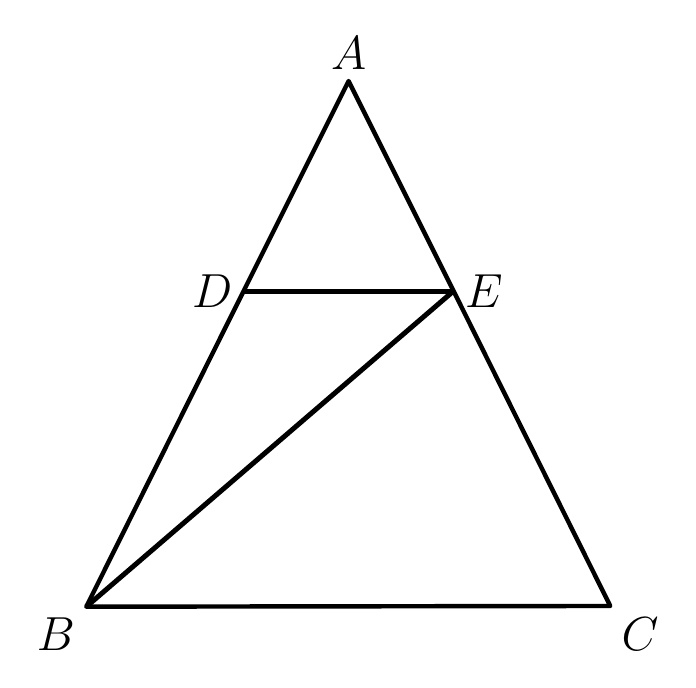
\begin{tikzpicture}[line width=1.6pt, line join=round]
\coordinate (A) at (-0.011,3.355);
\coordinate (B) at (-3.342,-3.321);
\coordinate (C) at (3.312,-3.312);
\coordinate (D) at (-1.344,0.688);



\coordinate (E) at (1.322,0.688);


\draw (A) -- (D) -- (B) -- (C) -- (E) -- cycle;


\draw[line width=1.8pt] (B) -- (E);
\draw[line width=1.8pt] (D) -- (E);


\node[above, font=\fontsize{17}{20.4}\selectfont] at (A) {$A$};
\node[below left, font=\fontsize{17}{20.4}\selectfont] at (B) {$B$};
\node[below right, font=\fontsize{17}{20.4}\selectfont] at (C) {$C$};
\node[left, font=\fontsize{17}{20.4}\selectfont] at (D) {$D$};
\node[right, font=\fontsize{17}{20.4}\selectfont] at (E) {$E$};
\end{tikzpicture}
\end{document}